%----------------------------------------------------------------------------------------
%	Metropolia Thesis LaTeX Template
%----------------------------------------------------------------------------------------
% License:
% This work is licensed under the Creative Commons Attribution 4.0 International License. To view a copy of this license, visit http://creativecommons.org/licenses/by/4.0/.
%
% Authors:
% Panu Leppäniemi, Patrik Luoto and Patrick Ausderau
%
% Credits:
% Panu Leppäniemi: abstract, def, cleaning,...
% Patrik Luoto: title page, abstract in Finnish, abbreviation, math,...
% Patrick Ausderau: initial version, style, table of content, bibliography, figure, appendix, table, source code listing...
%
% Please:
% If you find mistakes, improve this template and alike, please contribute by sharing your improvements and/or send us your feedback there: https://github.com/panunu/metropolia-thesis-latex
% And of course, if you improve it, add yourself as an author.
%
% Compiler:
% Use XeLaTeX as a compiler.

%----------------------------------------------------------------------------------------
%    ToDo
%----------------------------------------------------------------------------------------
% % % TÄRKEÄT
% % Odotetaan 29.11.2013 asti äikänmaikkojen ja viestinnän mahdollisia kommentteja.
%   %done?
%
% % % Vähemmän tärkeät
  % PNG:iden tilalle vektorigraffaa, jos vain löytyy kohtuuvaivalla

 
%----------------------------------------------------------------------------------------
%	THESIS
%----------------------------------------------------------------------------------------

\def\thesislang{english} %change this depending on your language
\author{Luong Nguyen Khoi Nguyen}
\def\thesis{Thesis}


%English section, for abstract
\title{Application of Protocol-Oriented MVVM Architecture in iOS Development}
\def\metropoliadegree {Bachelor of Engineering}
\def\metropoliadegreeprogramme {Information Technology}
\def\metropoliaspecialisation {Smart Systems}
\def\metropoliainstructors {
Patrick Ausderau, Senior Lecturer

Vu Nguyen, Instructor
}
\def\metropoliakeywords {\acrlong{mvvm}, \acrlong{pop}, Swift, Architecture, \gls{trait}, \acrlong{ios}}
\date{25 April 2017}

%----------------------------------------------------------------------------------------
%	GLOBAL STYLES
%----------------------------------------------------------------------------------------

\documentclass[11pt,a4paper,oneside,article]{memoir}
\usepackage[\thesislang]{babel} 
\usepackage{iflang}
\usepackage{amsmath}
\usepackage{amsfonts}
\usepackage{amssymb}
\usepackage{fontspec}
\usepackage{tocloft}
\usepackage{titlesec}
\usepackage[hyphens]{url}
\usepackage{mathtools}
\usepackage{wallpaper}
\usepackage{datetime}
\usepackage[bookmarksdepth=subsection]{hyperref} % for automagic pdf links for toc, refs, etc.
\usepackage[amssymb]{SIunits}
\usepackage[version=3]{mhchem}
\usepackage{pgfplots} %simple plots etc
\usepackage[justification=centering]{caption}
\usepackage{pgfplotstable}
\usepackage{tikz} % mindmaps, flowcharts, piecharts, examples at http://www.texample.net/tikz/examples/
\usetikzlibrary{shapes.geometric, arrows}

\renewcommand{\dateseparator}{.}
%condition for adding or not space in TOC
\usepackage{etoolbox}
%for compact list
\usepackage{enumitem}
%for block comment
\usepackage{verbatim}
%for "easier" references
\usepackage{varioref}
%forcing single line spacing in bibliography
\DisemulatePackage{setspace}
\usepackage{setspace}
%including figure (image)
\usepackage{graphicx}
%change the numbering for figure
\usepackage{chngcntr}
%strike trough
\usepackage{ulem}
%euro symbol
\usepackage{eurosym}
%try to count
\usepackage{totcount}
%insert source code
\usepackage{listings}
\usepackage[justification=justified,singlelinecheck=false]{caption}
\usepackage{color}
%force the width of a table instead of column
\usepackage{tabularx}
\usepackage{booktabs} %why not booktabs? :3
% Abbreviations, acronym and glossary
\usepackage[acronym,nonumberlist,section,nopostdot]{glossaries}%xindy,%toc, ,nomain

\usepackage{float} % For forced figure location with modifier H (\begin{figure}[H])
\usepackage{cite} % Make citations to match Metropolia thesis guide

% change font of links in bibliography to same as other text
\usepackage{url}

\urlstyle{same}

%Package for code listing
\usepackage{minted}

\usemintedstyle{xcode}


% change punctuation of multiple cites to semicolon instead of comma: [1; 2; 3]
\renewcommand\citepunct{; }

% citep-macro for reference with period inside square brackets [1.]
\newcommand{\citep}[1]{
 \renewcommand\citeright{.]}
 \cite{#1}
 \renewcommand\citeright{]}
}

%set date format to D.M.YYYY
\newdateformat{specialdate}{\THEDAY.\THEMONTH.\THEYEAR}

\newcommand\tn[1]{\textnormal{#1}} %use \tn instead of \textnormal
\newcommand\reaction[1]{\begin{equation}\ce{#1}\end{equation}} %\reaction{} for chemical reactions

%NORMAL TEXT
%all text, title, etc. in the same font: Arial
%replace with arial.ttf if you have the fontfile
%NOTE: fontname is case-sensitive
\setmainfont{LiberationSans}
%line space
\linespread{1.5}
%\doublespacing
%margin
\usepackage[top=2.5cm, bottom=3cm, left=4cm, right=2cm, nofoot]{geometry}
\setlength{\parindent}{0pt} %first line of paragraph not indented
\setlength{\parskip}{16.5pt} %one empty line to separate paragraph
%list with small line space separation
\tightlists

%IMAGE - FIGURE
%the figures should be placed in the "illustration" folder
\graphicspath{{illustration/}}
%figure number without chapter (1.1, 1.2, 2.1) to (1, 2, 3)
\counterwithout{figure}{chapter}
%border around images
\setlength\fboxsep{0pt}
\setlength\fboxrule{0.5pt}
%caption font size
\captionnamefont{\small}
\captiontitlefont{\small}
%space after figure caption (and other float elements)
\setlength{\belowcaptionskip}{-7pt}

%TABLE
\counterwithout{table}{chapter}

%Minted
\newminted[SwiftCode]{swift}{frame=single,bgcolor=lightgray,framesep=3mm,linenos,xleftmargin = 3mm,breaklines=true}

%SOURCE CODE
\definecolor{darkgray}{rgb}{.4,.4,.4}
\definecolor{lightgray}{rgb}{.94,.94,.94}
\definecolor{smokyblack}{rgb}{0.06, 0.05, 0.03}
\definecolor{purple}{rgb}{0.65, 0.12, 0.82}
\lstset{
extendedchars=true,
captionpos=b,
caption=\footnotesize,
basicstyle=\singlespacing\ttfamily,%\small\fontfamily{"Courier"}\selectfont,
keywordstyle=\color{blue}\bfseries,
commentstyle=\color{purple}\itshape,
identifierstyle=\color{black},
stringstyle=\color{red},
showstringspaces=false,
showspaces=false,
numbers=left,
numberstyle=\footnotesize,
numbersep=9pt,
tabsize=2,
showtabs=false,
xleftmargin=1cm,
breaklines=true,
breakatwhitespace=false,
}
\lstMakeShortInline[columns=fixed]|
\IfLanguageName {finnish} {\renewcommand{\lstlistingname}{Listaus}} {} % what is a good translation for this?
%\counterwithout{lstlisting}{chapter}
%moved after begin document, otherwise does not compile

%% set this format as the default for lstlisting
%\DeclareCaptionFormat{empty}{}
%\captionsetup[lstlisting]{format=empty}

%TOC
%change toc title
\IfLanguageName {finnish} {\addto{\captionsfinnish}{\renewcommand*{\contentsname}{Sisällys}}} {}
%remove dots
\renewcommand*{\cftdotsep}{\cftnodots}
%chapter title and page number not in bold
\renewcommand{\cftchapterfont}{}
\renewcommand{\cftchapterpagefont}{}
%sub section in toc
\setcounter{tocdepth}{2}
%subsection numbered
\setcounter{secnumdepth}{2}
\renewcommand{\tocheadstart}{\vspace*{-15pt}}
\renewcommand{\printtoctitle}[1]{\fontsize{13pt}{13pt}\bfseries #1}
\renewcommand{\aftertoctitle}{\vspace*{-22pt}\afterchaptertitle}
%spacing afer a chapter in toc
\preto\section{%
  \ifnum\value{section}=0\addtocontents{toc}{\vskip11pt}\fi
}
%spacing afer a section in toc
\renewcommand{\cftsectionaftersnumb}{\vspace*{-3pt}}
%spacing afer a subsection in toc
\renewcommand{\cftsubsectionaftersnumb}{\vspace*{-1pt}}
%appendix in toc with "Appendix " + num
\IfLanguageName {finnish} {
  \renewcommand*{\cftappendixname}{Liite\space}
  \renewcommand{\appendixtocname}{Liitteet}
}{\renewcommand*{\cftappendixname}{Appendix\space}}
%appendix header
\IfLanguageName {finnish} {\def\appname{Liite\space}}{\def\appname{Appendix\space}}

%TITLES
%chapter title
\titleformat{\chapter}
{\fontsize{13pt}{13pt}\bfseries\linespread{1}}
{\thechapter}{.5cm}{}
\titlespacing*{\chapter}{0pt}{.32cm}{9pt}
\titleformat{\section}
{\fontsize{12pt}{12pt}\linespread{1}}
{\thesection}{.5cm}{}
\titlespacing*{\section}{0pt}{14pt}{6pt}
\titleformat{\subsection}
{\fontsize{12pt}{12pt}\linespread{1}}
{\thesubsection}{.5cm}{}
\titlespacing*{\subsection}{0pt}{14pt}{6pt}


%QUOTE
\renewenvironment{quote}
  {\list{}{\rightmargin=0pt\leftmargin=1cm\topsep=-10pt}%
  \item\relax\fontsize{10pt}{10pt}\singlespacing}
  {\endlist}

%BIBLIOGRAPHY
%bibliography title to be "references"
%IF THE TITLE DON'T GET RENAMED PROPERLY, move that line after the \begin{document}
\IfLanguageName {finnish} {\addto{\captionsfinnish}{\renewcommand*{\bibname}{Lähteet}}} {\renewcommand\bibname{References}}
\makeatletter %reference list option change
\renewcommand\@biblabel[1]{#1\hspace{1cm}} %from [1] to 1 with 1cm gap
\makeatother %
\setlength{\bibitemsep}{11pt}

%count the appendices (since the chapter counter is reset after \appendix).
%! require to complie 2 times
\regtotcounter{chapter}

%ABBREVIATION AND GLOSSARY
% Generate the glossary
\makeglossaries

%Acronyms, abbreviations, etc. definitions
\newacronym{mvc}{MVC}{Model View Controller}
\newacronym{mvvm}{MVVM}{Model View View Model}
\newacronym{mvp}{MVP}{Model View Presenter}
\newacronym{pop}{POP}{Protocol Oriented Programming}
\newacronym{oop}{OOP}{Object Oriented Programming}
\newacronym{pop-mvvm}{POP MVVM}{Protocol Oriented Model View View Model}
\newacronym{tdd}{TDD}{Test Driven Development}
\newacronym{ios}{iOS}{iPhone Operating System}
\newacronym{kvo}{KVO}{Key-Value Observing}
\newacronym{wwdc}{WWDC}{Worldwide Developers Conference}
\newacronym{dry}{DRY}{Don't repeat yourself}
\newacronym{api}{API}{Application Programming Interface}
\newacronym{css}{CSS}{Cascading Style Sheets}
\newacronym{viper}{VIPER}{View Interactor Presenter Entity Router}
\newacronym{http}{HTTP}{Hypertext Transfer Protocol }
\newacronym{cpu}{CPU}{Central Processing Unit}
\newacronym{php}{PHP}{Hypertext Preprocessor}
%Glossary entries

\newglossaryentry{iOS}{
    name = iOS,
    description = {\acrlong{ios}: a mobile operating system created and developed by Apple Inc. exclusively for its hardware}
 }
 
 
\newglossaryentry{unit_test}{
    name = unit testing,
    description = {A software testing method in which a single logical unit is being tested to address potential issues
    }
 }
 
 \newglossaryentry{business_logic}{
    name = business logic,
    description = { Also known as domain logic, is a subset of the application logic whose main responsibility is to determine suitable operations on the data life cycle (creation, update, deletion, etc.) based on a real-world use case}
 }
 
 \newglossaryentry{trait}{
    name = Trait,
    description = { A design pattern often used in object-oriented programming, whose idea is to provide a set of functions with default implementation so that a class can use to extend its behaviours}
 }
 
 \newglossaryentry{interface}{
    name = interface,
    description = {In \gls{oop}, interface is a set of descriptions of actions that an object can do \cite{interface:definition}}
 }
 
 \newglossaryentry{singleton}{
    name = Singleton pattern,
    description = {A design pattern that restricts object creation. Only one object can be alive at a time and the pattern provides simple access to that object
    }
 }
 
\newglossaryentry{callback}{
    name = callback,
    description = {A function that is passed to a parameter list of another function and is triggered after some kind of event}
 }
 
 \newglossaryentry{json}{
    name = JSON,
    description = {Stands for JavaScript Object Notation, is lightweight data-interchange format. It is human readable, easy to parse or generate and language independent text format\cite{json:definition}}
 }
 
 \newglossaryentry{mit}{
    name = MIT,
    description = {A permissive software license, originally developed at the Massachusetts Institute of Technology \cite[p. 84]{mit:definition}}
 }
 
 \newglossaryentry{storyboard}{
    name = storyboard,
    description = {A visual presentation for screens inside the application and connections between them \cite{apple:storyboard}}
 }
 
 
\newglossaryentry{repository}{
    name = repository,
    description = {A place where data is being stored and managed}
 }
 
 \newglossaryentry{typealias}{
    name = typealias,
    description = {A named alias for an existing type, usually used for better convention \cite[p. 77]{apple:swift}}
 }
 
 \newglossaryentry{solid}{
    name = SOLID,
    description = {Abbreviation for: Single Responsibility, Open-Closed, Liskov substitution, Interface Segregation and Dependency Inversion, are the 5 basic principles for object-oriented programming development proposed by Robert C. Martin \cite[section II]{unclebob:agile}
    }
    
 }
 
 \newglossaryentry{first}{
    name = FIRST,
    description = {Abbreviation for: First, Isolated, Repeated, Self-validating and Timely, are the 5 basic principles for composing clean software testing proposed by Robert C. Martin \cite[p. 132]{unclebob:cleancode}}
 }
 
 \newglossaryentry{lifecycle}{
    name = lifecycle,
    description = {The series of changes in state of a UIViewController. \cite{apple:lifecycle}}
 }
 \newglossaryentry{appstore}{
    name = Apple App Store,
    description = {A digital distribution platform provided by Apple. It allows \gls{ios} users to browse and download applications developed with the development kit provided by Apple}
 }
 
 \newglossaryentry{managerclass}{
    name = Manager class,
    description = {A \gls{singleton} object which is restricted to operate on one and only one specific set of tasks (networking for example)}
 }
 
 \newglossaryentry{nodejs}{
    name = Node.js,
    description = {A platform built on JavaScript's runtime that uses an event-drivent and non-blocking I/O mechanism\cite{nodejs:definition}}
 }
 
 
%TITLE PAGE
\makeatletter
\renewcommand{\maketitle}{
\thispagestyle{empty}
\ThisCenterWallPaper{1}{viiva}
%
\vspace*{9.5cm}
\tn{\LARGE\@author\\[22pt]\Huge\IfLanguageName {finnish}{\otsikko}{\@title}\\[22pt]\LARGE\\[1.75cm]}

\parbox{.7\linewidth}{
\IfLanguageName {finnish}{
  Metropolia Ammattikorkeakoulu\\
  \tutkinto \\
  \kohjelma \\
  \thesis\\
  \pvm
} {
  Helsinki Metropolia University of Applied Sciences\\
  \metropoliadegree \\
  \metropoliadegreeprogramme \\
  \thesis\\
  \specialdate{25 April 2017} % D.M.YYYY date format
}
}
\ThisLRCornerWallPaper{1}{metropolia}
%
\clearpage
}
\makeatother

\makepagestyle{tiivis}
\makeevenhead{tiivis}{}{}{Tiivistelmä}
\makeoddhead{tiivis}{}{}{Tiivistelmä}

\makepagestyle{abstract}
\makeevenhead{abstract}{}{}{Abstract}
\makeoddhead{abstract}{}{}{Abstract}

\begin{document}
\counterwithout{lstlisting}{chapter}
\IfLanguageName {finnish} {\addto{\captionsfinnish}{\renewcommand*{\bibname}{Lähteet}}} {\renewcommand\bibname{References}}
\makeatletter %reference list option change
\renewcommand\@biblabel[1]{#1\hspace{1cm}} %from [1] to 1 with 1cm gap
\makeatother %
\setlength{\bibitemsep}{11pt}

%page number always on the top right, clear the "chapter/section" head
\pagestyle{myheadings}
\markright{}
%clear chapter "title" foot page
\makeevenfoot{plain}{}{}{}
\makeoddfoot{plain}{}{}{}

%----------------------------------------------------------------------------------------
%	TITLE PAGE
%----------------------------------------------------------------------------------------

\maketitle
\newpage
\LRCornerWallPaper{1}{footer}


%----------------------------------------------------------------------------------------
%	ABSTRACT
%----------------------------------------------------------------------------------------

\pagestyle{abstract}
\begin{tabular}{ | p{4,7cm} | p{10,3cm} |}
  \hline
  Author(s) \newline
  Title \newline\newline 
  Number of Pages \newline
  Date
  & 
  \makeatletter
  \@author \newline
  \@title \newline%\newline
  \pageref*{LastPage} pages + \total{chapter} appendices \newline %! if no appendices, risk to count total of chapter :D
  \IfLanguageName {finnish} {\foreignlanguage{english}{\longdate\@date}} {\@date}
  \makeatother
  \\ \hline
  Degree & \metropoliadegree
  \\ \hline
  Degree Programme & \metropoliadegreeprogramme
  \\ \hline
  Specialisation option & \metropoliaspecialisation
  \\ \hline
  Instructor(s) & \metropoliainstructors
  \\ \hline
  \multicolumn{2}{|p{15cm}|}{\begin{singlespacing}\vspace{-22pt}
  
  The mobile application industry is fast paced. Requirements change, additions of new features occur on a daily basis and demand frequent code structure adjustment. Thus, a flexible and maintainable software architecture is often a key factor for an application's success. The major objective of this thesis is to propose a practical use case of \acrlong{pop-mvvm}, an architecture inspired by the \acrlong{pop} paradigm.\newline
   
   This thesis explains the architecture concepts by analyzing the process of constructing a \acrlong{pop-mvvm}-oriented Swift application. Moreover, it indicates the uses of software development's best practices in specific situations. Drawbacks of modern architecture like \acrlong{mvc} are also addressed.\newline
   
   The main product of this thesis is a fully functional iOS application written in Swift. Also, for learning purposes, parts of the application's code base are extracted, modified and can be freely used under the \gls{mit} license.\newline
   
   In conclusion, the thesis exhibits how a well-design architecture could affect the overall quality of an application, especially in terms of maintainability. It also encourages a best-practice minded approach in software development and further studies toward the practical use of the \acrlong{pop-mvvm} architecture.
   
  \end{singlespacing}} \\[14cm] \hline
  Keywords & \metropoliakeywords
  \\ \hline
\end{tabular}
\clearpage

%----------------------------------------------------------------------------------------
%	Acknowledgement ?
%----------------------------------------------------------------------------------------
%\chapter*{Acknowledgement}
%Thanks to my cat
%\clearpage

%----------------------------------------------------------------------------------------
%	TABLE OF CONTENTS
%----------------------------------------------------------------------------------------

\makeevenhead{plain}{}{}{}
\makeoddhead{plain}{}{}{}
\pagestyle{empty} %remove page number in toc (if longer than 2 pages)
\tableofcontents*
\pagestyle{empty} %remove page number in toc (if longer than 1 pages)


\clearpage
%Uncomment this line if you do not have Abbreviations list.
%\pagestyle{plain}

%list of figure, tables comes here...


%----------------------------------------------------------------------------------------
%    Lyhenteet / Abbreviation
%----------------------------------------------------------------------------------------

\begin{singlespacing}

%PA: As soon as you have some abbreviations/glossary terms, delete/comment out that \glsaddall command
%\glsaddall

{
	\titleformat{\section}
	{\fontsize{13pt}{13pt}\bfseries\linespread{1}}
	{\thesection}{.5cm}{}
	%Adapt labelwidth (sorry for the ugly hack)
	\setlist[description]{leftmargin=!, labelwidth=5.5em}
	\IfLanguageName {finnish} {
		\printacronyms[title=Lyhenteet]
	}{
		\printacronyms[title=Abbreviations]
	}
	\setlist[description]{leftmargin=!, labelwidth=7em}
	\printglossary 
	\setlist[description]{style=standard} % reset settings back to default
}
\end{singlespacing}


\newpage

%page number always on top right; also for chapter "title" page
\pagestyle{plain}
\makeevenhead{plain}{}{}{\thepage}
\makeoddhead{plain}{}{}{\thepage}

\setcounter{page}{1} %page 1 should be Introduction
\ClearWallPaper
%----------------------------------------------------------------------------------------
%	CONTENT
%----------------------------------------------------------------------------------------

\sloppy % enforce alignment to fully justified

\chapter{Introduction}\label{introduction}
According to a monthly report conducted by Statista.com\footnote{\url{https://www.statista.com}}, as of June 2016, there have been around 2 million applications in \gls{appstore}\cite{market:prediction}. Compared to June 2015 when there was approximately 1.5 million units, it sees a 33\% growth \cite{statista:num_app}. The market is gradually growing and is expected to double in size by 2020 \cite{market:report}.


%(FIXED  
    %PA: Do you have a source/reference that support that claim? %NL: cited
    %PA: Is "Apple App Store" common knowledge? Or should you briefly describe it (create a new \newglossaryentry{app_store}{name and description} (check lines 270 - 280) and use the reference to it here with \gls{app_store}) 
    %PA: Here you must have the reference to the page from where we can get these numbers. Add an entry in the biblio.bib file and \cite{} that bibliography reference here. 
    %PA: eventually a \footnote{\url{Link to statista.com home page}} %NL: FIXED
    
    %PA: Do you have a source/reference with that last year prediction? Or was it coming from that same statista.com?
    %NL: can not find the source which claimed that. will replace with other predictions.
%)
 
The promising raise of \gls{ios} applications market results in a tougher battle for market shares. As pointed out in a white paper conducted by Intelliware, there are a number of critical factors that can make up a successful application \cite{intelliware:success}. Contributing to the likes of business value delivery, branding protection are application technical sides: optimization, scalability and extensibility. Undoubtedly, application growth is always an important element and needs to be arranged carefully during early stage of development. Moreover, Robert C. Martin once claimed that a software project's ability to respond to change plays a vital role in its success \cite[p.32]{unclebob:agile}. This implies the importance of constructing the application based on a testable, scalable and maintainable architecture \cite{architecture:architecsolution}.
%(FIXED? - fixed
    %PA: is this your claim? Is it comming from a book/article, if yes, reference \cite
    %NL: my opinion here. is ok or should I cite from a good source ?
    %PA: yes, if you have a source, it's always better
%)


Over the years, the \gls{mvc} architecture has been a popular choice among \gls{iOS} developers. As stated by Apple, \gls{mvc} is a good central design for \gls{ios} applications. It offers reusable codes, better defined interfaces and most importantly, a great cooperation with existing Cocoa technologies. However, the strict coupling between \gls{mvc}'s modules often poses a considerable drawback in the reusable aspect.\cite{apple:mvc} This problem is described as: when more data and \gls{business_logic} arrive, the View Controller module will be overloaded, neither reusable nor testable since it cannot be separated from the View. Thus, \gls{mvc} is often unabbreviated as Massive View Controller\footnote{This comes from the fact that View Controller is responsible for many tasks, hence grows expeditiously when the project evolves.}. As a result, a better defined pattern namely \acrfull{mvvm} is introduced.
%(FIXED
    %Should abbreviations be mentioned at first place, e.g: Model-View-Controller(MVC) ?
    %PA: Yes. Check around line 270. Create a new acronym \newacronym{id}{short}{full} there and here use the \gls{id} (as well as in every place where you mention it).
    %PA: should you define MVC (\newglossaryentry) or will you define it in the theory chapter?
    %PA: iOS is also an abbreviation and/or could also be defined (\newglossaryentry) %NL: FIXED
    %PA: so e.g. here you will use that same \gls{id} %NL: FIXED
    %PA: do you have a reference? Will you explain more that concept in the theory chapter? %NL:Explained later in theory
    %PA: this is also an abbreviation (create \newacronym). You then must define it in the theory chapter.  %NL: FIXED
%)

\gls{mvvm} offers an independent business domain called View Model which handles all the data transformation and operations. Since it is a standalone domain and not attached to any other layers, \gls{unit_test} is easily integrated. Moreover, with the emerge of \acrfull{pop} in recent years, View Model becomes more flexible and reusable when paired with a Trait-like design pattern \cite{machinethink:pattern}. This study aims to demonstrate the use of the \gls{pop-mvvm} architecture in developing a real-world \gls{iOS} application with the case study of Tintm\footnote{\url{https://www.tintm.com}}, a news aggregator application. Moreover, a number of practices that serve as illustrations for software development principles like \gls{solid} and \gls{first} will also be integrated in this study. 
%(FIXED
    %Should I mention the case study here ? %PA: Yes, that's ok. Maybe a longer explanation what this case study/application is in the theory chapter if needed?
    %PA:\gls %NL: FIXED
    %PA: maybe define "unit test" (either \newglossaryentry or in the theory chapter) %NL: FIXED
    %PA: abbreviation => \newacronym. Will you explain it in the theory chapter? %NL: FIXED. Explanation in theory
    %PA: maybe an explanation of all the combinations of MVC, view controller, view model,... in the theory chapter?
    %NL: yeah I think it is better to go into more details in the theory chapter, since intro should be limited to 1 page
    %PA: \gls
    %PA: maybe a footnote to the webpage of the app? %NL: done
%)
    
\newpage
\chapter{Theoretical Background}\label{theoretical}

%todo
\section{\acrfull{mvc}} %PA: I would go for \acrfull{mvc}. But do as you prefer (and be consistent).

First introduced in Smalltalk\footnote{One of the very first programming languages that support \gls{oop} paradigm, developed around the 1970s for educational purpose \cite{smalltalk:definition}} in the 1980s, \gls{mvc} quickly emerges as one of the most influential design pattern for rich graphical user interface application \cite{pope:mvc}. In \gls{ios} \gls{mvc} design pattern, objects in the application are grouped to 3 different layers: Model, View and Controller. They are separated from the others by some abstract borderlines. Communication between these layers is accomplished through these boundaries \cite{apple:mvc}.
%(FIXED
    %PA: check with English teacher, for me it sounds "introduced by someone". But here, Smalltalk is a thing (a programming language); should it be "introduced in" or "into"? #should be in, I fixed it
%)

\begin{figure}[h]

\centering
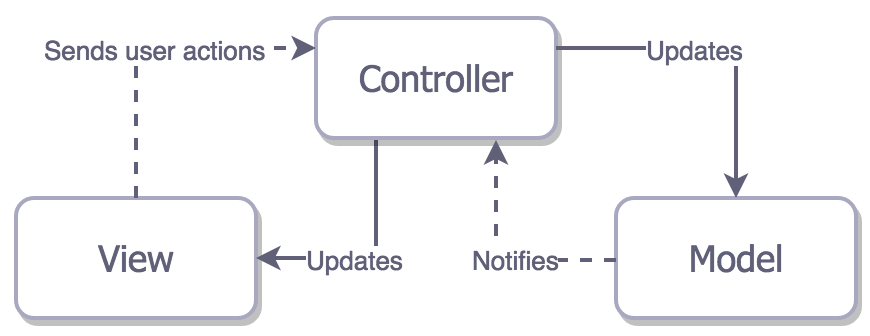
\includegraphics[width=\textwidth]{mvc}

\caption{MVC pattern (Reprinted from Orlov (2015) \cite{medium:pattern})}
\label{fig:mvc}
\end{figure}
%PA: check thesis guide again. Should be "reprinted from Author (year) \cite{}.". In this case "MVC pattern. Reprinted from Orlov (2015) \cite{medium:pattern}."
%PA: Check all figure for consistency.

%(FIXED (somehow)
    %PA: Figure must be referenced in the text! So somewhere appropriate there should be a sentence like "as seen in figure \ref{fig:mvc}" (this comes from the thesisGuide)
    %PA: Did you do the image yourself? If you copied and/or modified an existing image, you must have a reference in the caption like "MVC pattern (modified from John Doe 2015 \cite{some:id}" (this comes from the thesisGuide)
%)

Data encapsulation, computation and manipulation are done within the Model object. Persistent data and networking data also reside here. Ideally, Model must not have a direct connection with the View layer, since it should not be involved in user interaction operations.

View is the interaction point between users and the application. Its main responsibility is to display data stored in Model and enable editing for that data. Ideally, Model and View will communicate through a Controller as described in figure \ref{fig:mvc}. Nevertheless, as mentioned in chapter \ref{introduction}, they are often coupled.

Controller serves as the middle man between one or more models and one or more views. As described in figure \ref{fig:mvc}, there is a ruleset that indicates clear connections between specific domains. As an intermediary, Controller is the conduit through of the pattern in which changes in View or Model are learnt by the other. 
%(FIXED 
    %PA: E.g. in one of these sentences would be a good place to have the reference to the figure.
%)
User interaction made in View is interpreted by Controller which then notifies the changed state in data to the Model layer. Vice versa, any changes occur in Model object is recorded by Controller via \gls{kvo} system \cite{apple:kvo}, which in turn updates the data displayed by View. \cite{apple:mvc}

\section{\acrfull{mvvm}}\label{section:mvvm}
In mainstream Apple's \gls{mvc}, almost all the \gls{business_logic} is put into the Controller's body. \Gls{business_logic} often consists of: data operations on models, networking tasks, handlers for view's interactions, etc. In some cases, a part of the \gls{business_logic} can be offloaded to Model layer ( data calculation for example). On the other hand, the View's only responsibility is to send actions to the Controller. Thus, it makes the overall architecture imbalanced in term of responsibility division.

\begin{figure}[h]

\centering
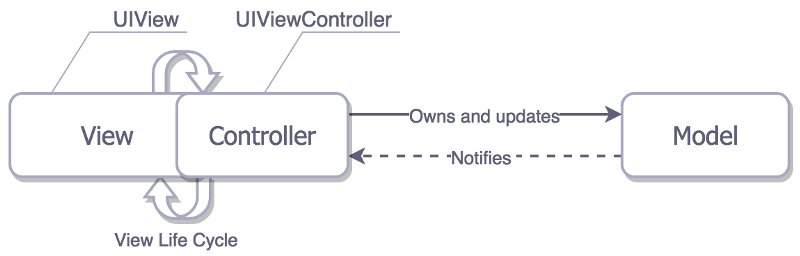
\includegraphics[width=\textwidth]{mvcInReality}

\caption{MVC in reality (Copied from Orlov (2015) \cite{medium:pattern})}
\label{fig:mvcInReality}

\end{figure}
%(FIXED
    %PA: same comments: figure must be referenced in the text. Is it your own image?
%)

In a real-world \gls{mvc}-based project, View is usually found to be coupled with its Controller as presented in figure \ref{fig:mvcInReality}. This coupling makes both component neither reusable nor testable. Moreover, Controller is easily overloaded and increases steadily in size when the application grows. Addressing the problem of overwhelmed Controller in \gls{mvc}, Microsoft introduced the \gls{mvvm} design pattern\cite{microsoft:mvvm}. Theoretically, \gls{mvvm} is an upgrade of Apple's \gls{mvc}, where the main components are kept and the domain logic is delegated to a new layer, namely View Model. 
 
The new states of View and Controller are illustrated in figure \ref{fig:mvvm}. They pair up and eventually become a unique domain. Controller does not hold reference to Model anymore, instead they communicate through View Model, the newly introduced layer. Having View Model as a middle man brings many benefits in terms of testing and expanding the application. Firstly, View Model forms a one-way communication with View by binding itself to the corresponding View. As a result, the View layer holds reference to its View Model but the View Model is restricted from knowing about its View. Thus, it can be widely reused and adopted by many different View objects.

%PA: at the very end, we will move the figure and switch to [h!] to avoid breaking paragraph.
\begin{figure}[h]

\centering
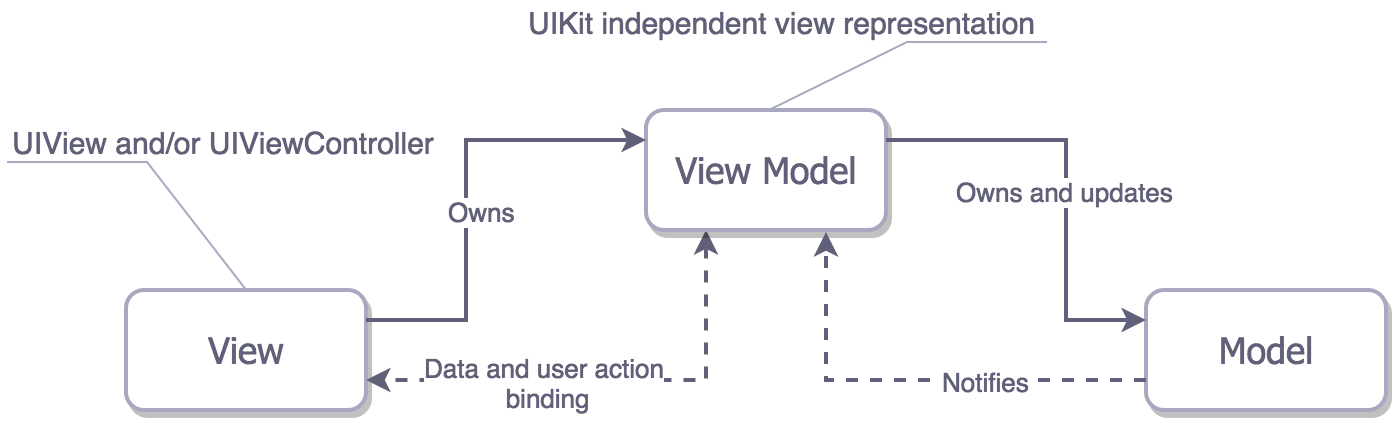
\includegraphics[width=\textwidth]{mvvm}

\caption{MVVM pattern ( Copied from Orlov (2015) \cite{medium:pattern})}
\label{fig:mvvm}

\end{figure}
%(FIXED
    %PA: same comments: figure must be referenced in the text. Is it your own image?
%)


Secondly, View Model is capable of observing changes in Model and synchronize itself with the events. Since there exists a binding between View and View Model, the former is therefore updated accordingly. This results in a responsive experience for users as well as forming a solid signalization system, where events occur inside each components are decoded as signals and bound to specific handlers.\cite{microsoft:mvvm}

Finally, \gls{unit_test} in \gls{mvc} is often an issue. Most of the \gls{business_logic} code usually resides within the View Controller which makes it the only possible place to perform \gls{unit_test}. A View Controller's state changes throughout its \gls{lifecycle} and the same goes for the Model it possesses. When the Model's state is dependent on the UI environment, \gls{unit_test} becomes trickier since side-effects is bound to happen during the test therefore leaving the test output unverified. Consequently, additional step is required in order to isolate the Model's state so as to prevents UI environment from changing it. 

However, in \gls{mvvm}, View Model is an UI-independent layer. Reference to Controller is eliminated and as a result, Model remains isolated. Performing \gls{unit_test} upon View Model is thus made easier. Also, little effort is invested in preparation and neglecting side-effects. 

%(FIXED:
    %PA: Can you manage without the bullet list? This is almost a paragraph. (yes, whenever you can, avoid bullet list (this comes from the thesisGuide))
    %PA: check with English teacher, they don't like the shortened form...
    %LNKN: what do you mean by shortened form? Is it View Model instead of View Model ?
    %PA: "sync" is the short form for "synchronize"; but since it's the dictionary since the 1930's, I guess the English teacher may accept it.
%)

\section{\acrfull{pop}}\label{section:pop}
\gls{pop} %PA: you already have {pop} in Introduction chapter, so you can go for \gls{pop}. And if you change to \acrfull{} in section, you would have the "reminder" of the full name and abbreviation.
is a programming paradigm which was introduced by Dave Abrahams at the \gls{wwdc} in 2015 \cite{pop:wwdc}. %PA: "at the wwdc in 2015"
In contrast to \acrfull{oop} %PA: First time seen in the text (if we ignore the glossary). Maybe switch to \acrfull{oop} (or check with English teacher)
whose idea is based on the concept of object\footnote{An unit that encapsulates data and owns the corresponding accessors for that data.} \cite{lafore:oop}, \gls{pop} focuses on the use of protocols. \gls{pop} in fact is not considered as a preferable paradigm for Swift but more of an enhancement for \gls{oop}. Its adoption helps solve many disadvantages \gls{oop} has long introduced as well as playing a vital role in improving code base flexibility, scalability and testablity that many \gls{oop}-based Swift projects lack. 

\subsection{Protocol}
A protocol in Swift is an \gls{interface} that provides specific methods. Any object conforms to that protocol must implement the given set of functions. %PA: second half of the sentence is not very clear. consider reformulating.
According to Apple's documentation: ``A protocol defines a blueprint of methods, properties, and other requirements that suit a particular task or piece of functionality'' \cite{apple:protocol}.
%LNKN: is this a correct way of directly quoting a definition?. %PA: yes. but put a space after colon
%PA: text double (or single) quote in latex is achieved with the backquote to open and "normal" single quote to close (and double them for double quote). ``some copied text here'' that will print with the right curly quote based on the language.
The takeaway point is that a protocol is a blueprint, that is, something that gives instructions but no particular implementation. In other words, a protocol represents actions, indicates how an object can act. As a result, it provides developers with a convenient method of extending an existing object's behaviours, while reducing the overhead of expanding base classes' functionality through the act of inheriting. Moreover, protocols can be widely adopted by classes, structures and enumerations \cite[p .41]{apple:swift} thus simplifying writing codes in many cases. For example, any class that conforms to an Error protocol could provide its own implementations for error handling. 

\begin{listing}[H]
\begin{SwiftCode}

enum SignupError: Error {
    case invalidPassword
    case invalidUsername
    case emptyField
}

do {
    try signUp(username: "Nguyen", password: "abcd")
} catch SignupError.invalidPassword {
    print("Password must be longer than 8 characters.")
} catch SignupError.invalidUsername {
    print("Username is alreadyTaken.")
} catch SignupError.emptyField {
    print("Some fields cannot be empty.")
}
\end{SwiftCode}
\caption{Example of using Error protocol in Swift}
\label{swift:errorprotocol}
\end{listing}

Characterizing errors by grouping them into enumerations greatly enhances code readability. Moreover, not only objects can supply their own error handlers as shown in listing \ref{swift:errorprotocol}, but they can adopt the default implementations provided by protocols they conform to. This scenario will be explained in section \ref{protocolextension}.
%LNKN: Can I give some code pieces here for demonstration purpose ? %PA: yes; why not. Then you will have to reference it in the text like for figures/tables and explain what the code do.


\subsection{Protocol Extension}\label{protocolextension}
In many programming languages, the protocol is restricted from having its own implementation. In contrast, Swift allows a protocol to fulfill its methods by using extension. Not only extension can add functionality to protocols, the same applies to classes, structs and enumerations \cite{apple:extension}.

By extending a protocol, all of its conformance will be eligible to use the default implementations defined inside the extension. As mentioned in section \ref{section:pop}, \gls{pop} favours the use of the protocol over the class. Hence, \gls{pop}-based projects are often built upon the foundation of protocols. With extensions, protocols can grow and expand without paying extra attention on the compatibility %PA: typo?
of existing codes. Furthermore, any types that conform to such protocols will therefore take affect %PA: maybe check with English teacher: https://www.vocabulary.com/articles/chooseyourwords/affect-effect/
as a whole, reducing the need of modifying implementations individually when requirements change.

\subsection{Trait-like pattern in \gls{pop}}
\Gls{trait} is a concept that has been adopted by many programming languages with the likes of Scala, Groovy, \gls{php}\footnote{Eventually, Trait is  reserved as a keyword in those languages \cite{scala:trait, groovy:trait, php:trait}.}, etc. Not until the introduction of protocol extension that \gls{trait} officially becomes available in Swift. The spirit of \gls{trait} lies behind the idea of extending a class functionality without having it inherits from some other classes. This feature proves to be powerful in many situations, especially in the cases of programming languages that do not support multiple inheritance. The comparison between a trait and a protocol is displayed in figure \ref{fig:interfaceVsTrait}. 

\begin{figure}[H]


\centering
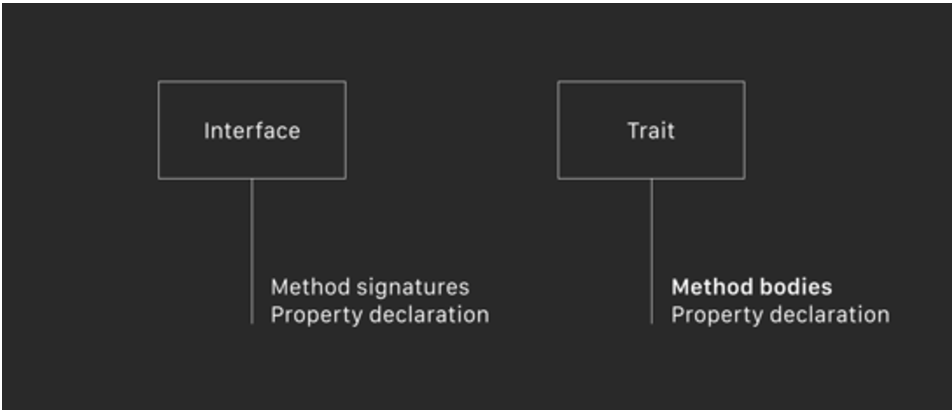
\includegraphics[width=\textwidth]{interfaceVsTrait}

\caption{Interface vs Trait (Modified from Matthijs Hollemans (2015)\cite{machinethink:pattern})}
\label{fig:interfaceVsTrait}


%LNKN: is there anyway we can put the figure at the end of page 7? Now it is placed at the top of page 8. %PA: You have to use the [h!] flag. But we do it at the very end of the thesis. Let them float around for now.
\end{figure}

It is noteworthy that while \gls{interface} only provides class with method signatures, \gls{trait} also offers the method bodies as presented in figure \ref{fig:interfaceVsTrait}. Naturally, using the protocol with extension is the way Trait-like pattern is applied in Swift. As a pattern that supports factoring hierarchies and encourages code reusability \cite{typed:trait}, \gls{trait} is an essential part in an \gls{pop} based application. 

\subsection{Using \acrfull{pop} in Swift}
Given that \gls{pop} is still a relatively new paradigm, one can ponder over the practical use of \gls{pop} in Swift development. In fact, there are numerous reasons to support the idea of \gls{pop}. Firstly, most of the times, it is good practice to adopt the ideas that are implemented at the heart of a language. As claimed by Dave Abrahams at the \gls{wwdc} in 2015, Swift is a protocol-orieneted language \cite{pop:wwdc}. An observation on the distribution of classes, structures and enumerations inside Swift's standard library will clarify that claim.

%PA: Why figure??? Use listing! This is your "simple script"! For example:

\begin{listing}[H]
\begin{SwiftCode}
Nguyens-MacBook-Pro:swift_stdlib-master nguyenluong$ grep -e "^protocol" stdlib.swift | wc -l
      73
Nguyens-MacBook-Pro:swift_stdlib-master nguyenluong$ grep -e "^struct" stdlib.swift | wc -l
      87
Nguyens-MacBook-Pro:swift_stdlib-master nguyenluong$ grep -e "^class" stdlib.swift | wc -l
       4  
\end{SwiftCode}
\caption{Using Bash script to  display number of protocols, struct and class used in Swift standard library}
\label{simple:script}
\end{listing}

%If needed reduce space after with \vspace{-17pt}
%And then refer to it like "as seen in listing \ref{simple:script} blah blah..."

As observed in listing \ref{simple:script}, there are 87 structs, 73 protocols and only 4 classes reside in Swift's standard libraries. This result clearly reaffirms Abrahams' statement on the paradigm Swift is following. Moreover, one big drawback of \gls{oop} is the scalability of its inherent system. An \gls{oop}'s based application is built upon classes and inheritance structure. When a class inherits from another, it has the rights to use the properties and methods defined in the base class and therefore reducing the need of creating its own implementation. However, it is worth noticing that in a majority of programming languages a class can only inherit from a single base class. Thus when the project grows, there appear three possible problematic consequences:

\begin{enumerate}
  \item Base classes are overloaded with additional functionality if no new class is created to share the responsibilities.
  \item New classes are added and the hierarchy tree will grow even deeper hence reduce abstraction level.
  \item In many cases, classes may have the behaviours of two or more base classes.  Inheritance limits their chance to pick up implementations from other classes.
\end{enumerate}

To illustrate the aforementioned claims, the study will demonstrate a case study taken from an article written by Matthijs Hollemans\cite{machinethink:pattern}. This case clarifies the beneficial factors of applying \gls{pop} concept into a Swift project by analysing the state of a project before and after \gls{pop} is involved. 

\begin{figure}[H]
\centering
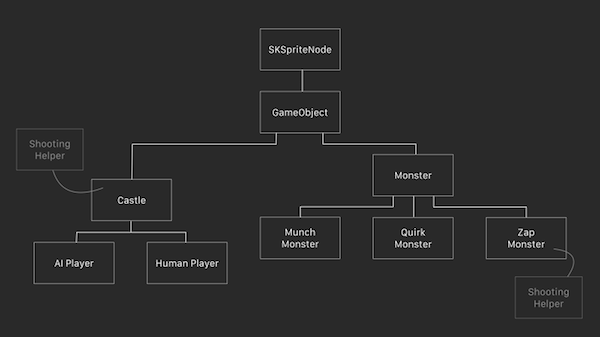
\includegraphics[width=\textwidth]{beforePop}

\caption{Hierarchy tree of an \gls{ios} game (Copied from Matthijs Hollemans (2015) \cite{machinethink:pattern})}
\label{fig:beforePop}
\end{figure}

The hierarchical structure of an iOS game is illustrated in figure \ref{fig:beforePop}. It contains a SKSpriteNode class which acts as the root of the hierarchy. Furthermore, there exists multiple classes that inherit from their descendants. Additionally, there are two helper classes responsible for enhancing the class' default behaviour. As observed from figure \ref{fig:beforePop} %PA: must have \ref{}
, the hierarchy tree can grow to a complex stage and become divergent along the growth of the project. Moreover, considering a situation where a newly added class requires behaviours of both Castle and Monster class, it results in  difficulty regarding the choice for base class. To overcome such problems, \gls{pop} servers as a handy tool. By making every class conform to protocols, the deep, nested, complicated hierarchy tree in \ref{fig:beforePop} is flattened into a clean and simple one as described in figure \ref{fig:afterPop}. %PA: Always figure number!

\iftrue
\begin{figure}[H]

\centering
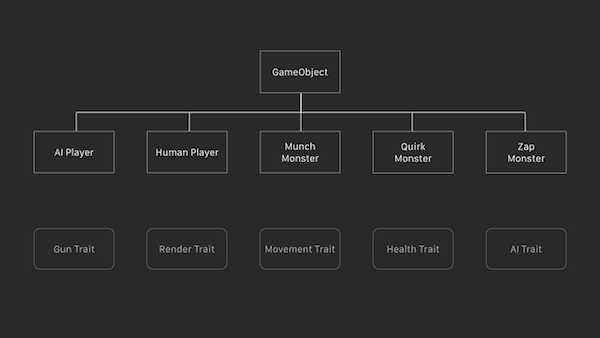
\includegraphics[width=\textwidth]{afterPop}

\caption{Hierarchy tree of an \gls{ios} game after applying \gls{pop} (Copied from Matthijs Hollemans (2015) \cite{machinethink:pattern})}
\label{fig:afterPop}

\end{figure}
\fi

The original idea of \gls{pop}\footnote{See section \ref{section:pop}}, which is to reduce the need of inheritance as much as possible, is well displayed in this situation. Firstly, relative behaviours are grouped into protocols. Then, the protocols are bound to their own extensions. Finally, default implementations are generated within the extension, thus form multiple \glspl{trait}. Classes can now choose which types of behaviours they want to own instead of being restricted by the set of actions that their parent classes provide. An explanation for this transformation is described in the following order.

A Munch Monster can move and shoot, a Zap Monster can move and shoot too but a Quirk Monster can only move. Unfortunately, as of figure \ref{fig:beforePop} shows, the Monster class they inherit from only offers the movement ability, which means that Zap Monster and Munch Monster class will have to implement the shooting ability on their own. Another possibility is that the shooting ability can be added directly to the Monster class. However, the addition becomes unnecessary %PA: "redundant" (= repetition) is not the best word. If I understand corecetly, here you want to say "too much" because the Quirk don't need it. %LNKN: changed to "unnecessary"
because the Quirk Monster class does not need it. \\
By creating \glspl{trait} for different abilities, the Monster's child classes can select the types of \gls{trait} they want to conform to. Given that each trait comes with their own implementations, the conformance would require little to no additional specifications for their behaviours. As a paradigm that favors composition over inheritance, \gls{pop} is a great enhancement for the classic \gls{oop}, especially in term of neglecting code's redundancy and inheritance complexity in development. 

\section{\acrlong{pop-mvvm} Architecture} 
One considerable advantage when adopting the \gls{mvvm} structure is the isolation of business logic. However, in reality, it is difficult to observe this benefit due to the specific binding between Controller and View Model objects. By definition, View Model is a unit that packs all domain logic a Controller needs. Henceforth, a View Model is only reusable in the case where there are 2 or more Controllers share a same package of functionality, which rarely happens in a real-world project. However, this problem can be solved by having View Model conforms to a number of different \glspl{trait}.

    \iftrue
    \begin{figure}[H]
    
    \centering
    \includegraphics[width=\textwidth]{pop-mvvm}
    
    \caption{Comparison of \gls{mvvm} pattern and \gls{pop-mvvm} pattern}
    \label{fig:pop-mvvm}
    
    \end{figure}
    \fi
    
Views are unique in terms of responsibilities and the same applies to their View Models. Although it is very unlikely to observe two identical View Models, having two or more of them sharing some functionality is common. If these View Models have completely separated implementations, they may violate the \Gls{dry} rule\footnote{The rule states that: ``Every piece of knowledge must have a single, unambiguous, authoritative
representation within a system.''\cite[p. 46]{andrew:pragmatic}}, thus reducing code reusability. The View Models in figure \ref{fig:pop-mvvm} encapsulates interactions one can have with their pets. However, either it is a cat or a dog, the way they are fed or played with appears to be the same. Consequently, it is not efficient to write a same logic twice. 

The right-hand side of figure \ref{fig:pop-mvvm} displays the state of the project after \gls{pop} is applied. These interactions are split into multiple traits, e.g: Feeding \glspl{trait}, Playing \glspl{trait}, etc. Instead of defining their own implementations, View Model can conform to these \glspl{trait}. This practice greatly reduces the number of duplicated implementations in View Models since each \gls{trait} has their own logic defined already. Furthermore, \gls{pop} considerably enhances the code structure in term of flexibility. For example: number of interactions with the pets may increase in the future. The owner can have them clean the home, feed the kids etc. Basically, without \gls{pop}, these interactions need to be redefined in each and every View Model. Behaviour \glspl{trait} provided by \gls{pop} not only avoids this hassle but also provides foundational implementations that new objects can easily make use of.

%FIXED (
    %PA: I understand what you mean; but is "on the contrary" too much? You already have "Although" at beginning of the sentence to mark the difference. 
    %PA: \newacronym{} and \gls{}
    %PA: \ref{}. But here, consider merging with the previous sentence to avoid repetition
 %)
    

\newpage
\chapter{Application}

\section{Description}

The project was carried out on request of SmartApp, a startup company based in Ho Chi Minh City. It was divided into two parts: front-end application and server side implementation. I was in charge of implementing the \gls{ios} application while the server-side part was done by another developer. The application flow is displayed in figure \ref{fig:workflow}.

\begin{figure}[h]

\centering
\includegraphics[width=\textwidth]{workflow}

\caption{Tintm's application flow}
\label{fig:workflow}

\end{figure}

The application aims to present its users the most popular news. For that reason, it is essential to construct a logical and efficient information filtering system. Firstly, articles are gathered from multiple reliable newspaper and sent to a news aggregator as observed from figure \ref{fig:workflow}. Then, inside the system, they are sorted and ranked based on multiple factors, for example: user views, social media interactions, published date, etc. Finally, the system outputs the refined data which will be displayed in an \gls{iOS} application. User interactions with the application are recorded and sent back to the aggerator system. Based on the records, the system can learn more about its users, study their behaviours and criteria. Consequently, its ranking mechanism improves gradually over time and serves better news which closely suit users' needs. 

\section{Development Process}
At the beginning of the development process, the team decided to use Waterfall methodology for this project. As a sequential model, each step in the Waterfall process must be fulfilled before the next step can begin. Furthermore, each step must also be verified to make sure that it complies with the requirements.\cite{waterfall:rumania} The process is straightforward and contains no iteration which makes it a viable choice for short time-span project like this ( 3 months). 
\begin{figure}[H]

\centering
\includegraphics[width=\textwidth]{waterflow}

\caption{Waterfall process}
\label{fig:waterfall}

\end{figure}

As seen in figure \ref{fig:waterfall}, a typical flow of Waterfall methodology often contains 5 stages. The first step was conducted in the first two weeks of the development process. In Waterfall methodology, it is essential that requirements are clear, concise and well understood by all the parties involved. Accordingly, the planning phase often takes more time than in other methodologies. \cite{waterfall:rumania} The design phase was carried out with the involvement of me and a designer and was completed within a week. The implementation phase was planned to be fulfilled in 2.5 months but unfortunately the deadline was not met due to some severe bugs. As a result, the development time had to span to a total of 5 months. The implementation phase took an additional month while verification and maintenance required another month to due. After that, project maintenance was carried out monthly and verified by the team leader.

\section{\gls{solid} as a Design Guideline}
As addressed by Robert Martin, one of the main causes for rotting software is constant requirement changes. These changes are often made quickly by the developers who are not familiar with the design philosophy. Thus over time, the initial design is violated and software quality starts to degrade. \cite[chapter 7]{unclebob:agile}

However, changes are unavoidable in software development and should not be the one to blame. An ideal design needs to be non-volatile and remains clean as changes come in. Moreover, it should be well protected from rotting and flexible enough for continuous changes. The practices to achieve such system are encapsulated in \gls{solid} principles. \cite[chapter 7]{unclebob:agile} With the hope of reducing code complexity, keeping a cohesive design and maintaining a robust code base, the application adopts \gls{solid} principles as its system design guideline. It involves classes and functions design , frequent integration of unit tests, etc. 

\section{Technologies}
The client application was written in Swift. Although Objective-C is also a reasonable choice for \gls{ios} development, Swift was the more favorable for this project. Reasoning for this choice is carried out in section \ref{discussion:swift}. 

The backend application was built by \gls{nodejs}. Renowned for the ability of building fast and scalable server application, \gls{nodejs} is a reasonable choice for server-side building. Taking advantages of its non-blocking mechanism ( also known as event-driven architecture)\footnote{A mechanism that allows codes to run without blocking execution of others. Detailed explanation is located at \gls{nodejs} official documentation \cite{nodejs:nonblocking}.}, \gls{nodejs} effectively boosts its performance as well as optimizes its throughput.\cite{herron:nodejs} Also thanks to the non-blocking I/O model, \gls{nodejs} can concurrently handle multiple connections, make it an excellent candidate for data-intensive and real-time applications \cite{holmes:gettingmean}. A simple benchmark between \gls{nodejs} based server and \gls{php} based server is taken to justify the aforementioned claims. Its result is illustrated in figure \ref{fig:nodejsvsphp}.

\begin{figure}[H]

\centering
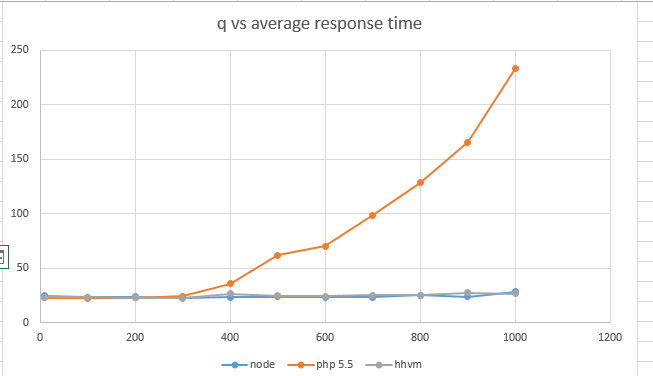
\includegraphics[width=\textwidth]{nodejs-vs-php-performance}

\caption{\gls{nodejs} vs \gls{php} \gls{http} and \gls{cpu} benchmark (Copied from Roberto Sanchez ( 2016)\cite{roberto:nodejs})}
\label{fig:nodejsvsphp}

\end{figure}

The test aims to compare \gls{http} and \gls{cpu} capabilities of both frameworks by making them execute bubble sort algorithm for a definite amount of input. The outcome from figure \ref{fig:nodejsvsphp} shows that \gls{nodejs}' performance is clearly ahead of \gls{php} when the amount of input increases: nearly ten times faster when the input consists of 1000 elements. Since the focus of this study is on the iOS development, \gls{nodejs}' productivity and performance will not be further discussed.

\newpage
\chapter{Implementation}
\section{Project Structure}
\subsection{ \Gls{mvvm} block} \label{section:mvvmblock}
The project structure is built upon the foundation of multiple Model-View-View Model combinations. For better convention, these combinations will be denoted as "blocks" from now on. Each block strictly follows \gls{mvvm} design principles \cite{microsoft:mvvm}. In addition, they also adapt to \gls{pop} paradigm, thus form a more advanced architecture namely \acrfull{pop-mvvm}.

\begin{figure}[H]

\centering
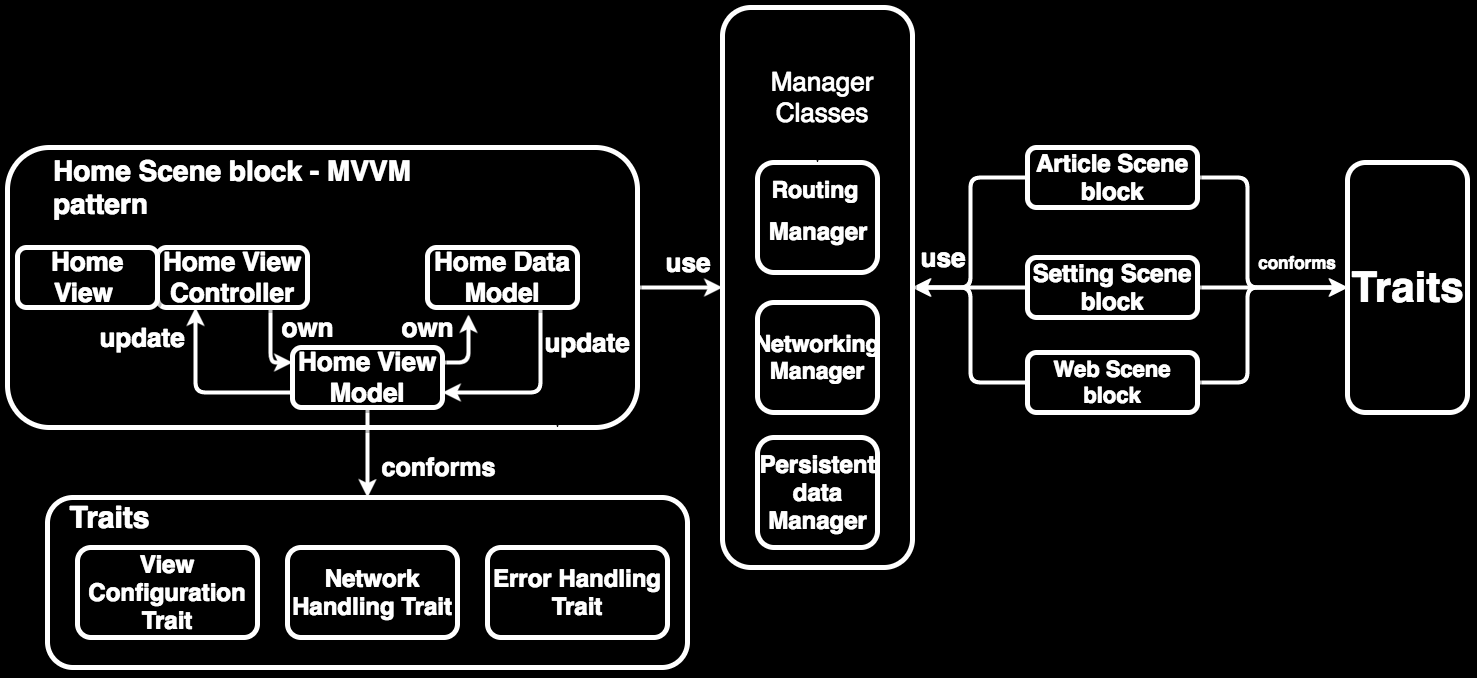
\includegraphics[width=\textwidth]{project-structure-diagram}

\caption{Project structure diagram}
\label{fig:projectStructure}

\end{figure}

The components inside each block establish their connections through a binding mechanism as mentioned in section \ref{section:mvvm}. As seen in figure \ref{fig:projectStructure}, a Model is bound to a View Model. Likewise, View Model is bound to a View Controller. These relationships are called one-way bindings \cite{microsoft:databinding}, where the inner object does not know anything about its owner. On the other hand, changes made within an inner object will be recognized by its owner through \gls{kvo} system. Since all units adopt the same architecture, only the construction for Home Scene block will be discussed in detail. 

\subsection{The inclusion of \glspl{trait}}
 As described in section \ref{section:mvvm}, the workload for View Model appears to be heavy since it is an isolated logic domain. View Model is responsible for processing networking data, exposing required information to View, catching and handling errors, etc. However, the appearance of \glspl{trait} in this architecture helps offload a significant amount of work for View Model. \glspl{trait} contain a set of features as well as basic implementations for them. By conforming to these Traits, View Model does not need to setup everything from scratch since they can use the existing solutions or modify them to suit their own needs.

There are a number of different \glspl{trait} being used in this project. For better convention, they are named after their unique responsibility. For example, a \gls{trait} responsible for Label View configuration is called Label Presentation Trait. In the same manner, Trait used for Image View setup is named Image View Presentable. For the sake of this study, only two aforementioned Traits will be discussed in detail in section \ref{presentationtraits}.

\subsection{Manager Classes}
For better abstraction, this project uses a number of Manager classes. Moreover, since related implementation details are wrapped into respective class and isolated from outside objects, it is easier to investigate bugs or potential flaws in the future. Nevertheless, there exists debates among the use of Manager class in software development. Thus, overusing is not encouraged\footnote{More information regarding the debate can be found at: \url{https://blog.codinghorror.com/i-shall-call-it-somethingmanager/}}.

In \gls{mvc} based Swift projects, navigation between scenes is often done within View Controller component \cite{apple:mvc}. However, it is not the case in \gls{pop-mvvm}. As shown in figure \ref{fig:projectStructure}, blocks do not communicate directly with the others, instead the communication is accomplished in a Routing Manager. This class takes care of creating necessary View and View Model objects, handling navigation transition animation and performing the navigation. In other words, Routing Manager's main responsibility is to glue all the blocks together. Such setup is inspired by another renowned \gls{ios} architecture namely \gls{viper}\footnote{This architecture is complex and only applicable in large scale project. More information concerning its implementation can be found at \url{https://www.objc.io/issues/13-architecture/viper/}}.

Networking Manager plays a vital role in almost every \gls{ios} application since it is the bridge between client and server applications. All operations relate to data from remote system should reside here, some of which include: making requests for data, constructing required parameters for requests, processing responses from server, etc. Processed data will be further manipulated inside responsible View Model via a \gls{callback} method.

Finally, as one goal of this project is to offer users offline reading ability, data persistence needs to be taken into consideration. After fetching articles from server, the application will attempt to store them into device's database. Persistence Data Manager utilizes all device's storage related operations. It can request access to the device's database and perform read, write, update or delete function there. The application uses Realm for data persistence due to its simple and modern features set\footnote{\url{https://github.com/realm/realm-cocoa}}.

\section{Implementation in detail}
As affirmed in section \ref{section:mvvmblock}, this study restricts detailed explanations for Home View, Home Controller and Home View Model. The study focuses on the manipulation of \gls{mvvm} architecture and \gls{pop} paradigm, therefore, Manager classes implementations will not be described.

\subsection{Home Scene Description}
Home Scene serves as the entry point of the application. It greets users with multiple lists of articles, sorted into respective categories. For better illustration, a blueprint of this scene is displayed in figure \ref{fig:homeSceneDescription}.

\begin{figure}[H]

\centering
\includegraphics[width=250pt]{homeSceneDescription}

\caption{Home scene blueprint}
\label{fig:homeSceneDescription}

\end{figure}

As observed from figure \ref{fig:homeSceneDescription}, Category A is selected since its background color differs from the others. Therefore, the articles below will belong to that category. At top of this scene lies a navigation bar which represent the list of categories. Users can navigate to different sections by sliding leftward or rightward.  Accordingly, the list of articles will also change. Each article contains a thumbnail, a title and a brief description. The design for this scene is kept as minimal as possible so as to improve the overall performance and avoid the user's distraction.

\subsection{Home Model}
The Home Model object wraps up necessary data for an article displayed in Home Scene. A diagram for this class is illustrated in figure \ref{fig:homeEntity}.

\begin{figure}[H]

\centering
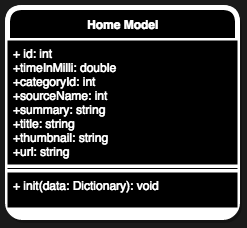
\includegraphics[width=200pt]{home-entity}

\caption{Home model diagram}
\label{fig:homeEntity}

\end{figure}

The parameters in figure \ref{fig:homeEntity} are self-explanatory already. Some notable variables are: 
\mintinline{swift}{id, categoryId, title, thumbnail} and \mintinline{swift}{summary}. First of, \mintinline{swift}{id} variable denotes a unique identification for the article. It will be used to fetch news' content later. \mintinline{swift}{CategoryId} specifies the identification of the category which this article belongs to, for example: Sport category has the id of 1, Politic's id is 2 etc. \mintinline{swift}{title} and \mintinline{swift}{summary} contain the article's headline and brief summary respectively. Finally, \mintinline{swift}{thumbnail} is a URL string which the application uses to download the thumbnail image for that article. Apart from the above variables, there is an initialization method in this class namely \mintinline{swift}{init} whose configuration is explained in listing \ref{swift:init}. 

\begin{listing}[h]
\begin{SwiftCode}
mutating func mapping(map: Map) {
        id <- map["Id"]
        categoryId <- map["CategoryId"]
        categoryName <- map["CategoryName"] 
        content <- map["Content"]
}
\end{SwiftCode}
\caption{Initialization method of Home Model}
\label{swift:init}
\end{listing}

This method processes raw data fetched from server, which is often a \gls{json} string. It does a simple operation: mapping values stored in a \gls{json} string into the object as shown in listing \ref{swift:init}. The value of key \mintinline{swift}{CategoryId} is mapped into \mintinline{swift}{categoryId} variable, \mintinline{swift}{Id} is mapped into \mintinline{swift}{id} variable and so on.

\subsection{Home Controller}
Home Controller is responsible for the user interface control. It captures user's interactions and vice versa, reflects changes in Home Model to user. Unlike in \gls{mvc} where Controller has to provide actions for these updates itself, the handlers are put in View Model. Therefore, Home Controller only has to signal Home View Model about user interactions and requests updated data from it as well.

\begin{figure}[H]

\centering
\includegraphics[width=\textwidth]{home-controller-diagram}

\caption{Home Controller diagram}
\label{fig:homeController}

\end{figure}

Home Controller is minimal and its only responsibility is to hold a View Model object as seen in figure \ref{fig:homeController}. Everything relates to UI configuration and View Model conformance is accomplished inside the \gls{storyboard} or delegated to Home Controller Delegate class. There are 2 Home Controller Delegate components which live within the app but for demonstration purpose, they aggregate to form a single class in figure \ref{fig:homeController}. The intent of splitting Home Controller functionality to multiple Delegate class is to satisfy the Single Responsibility Principle\footnote{The first principle in \gls{solid} which states that: ``A class or module should have one, and only one, reason to change'' \cite{unclebob:agile}}. 
According to the principle, each class or extension should only be responsible for one functionality, whether it is setting up UI attributes or handling data from View Model. 

\subsection{Home View Model}
Being the data \gls{repository}, Home View Model is in charge of refining data from multiple sources (server, device's database, etc.) as well as performing data binding between Home Model and Home Controller. Additionally, it also holds the necessary configuration for UI components inside Home Controller.

\begin{figure}[H]

\centering
\includegraphics[width=\textwidth]{home-view-model-diagram}

\caption{Home View Model diagram}
\label{fig:homeViewModel}

\end{figure}

Apart from holding an array of Home Model objects, Home View Model also owns a delegate property as shown in figure \ref{fig:homeViewModel}. This object contains a set of \gls{callback} functions and acts as a communication protocol between View Model and the Controller it binds to. As illustrated in listing \ref{listing:viewModel}, Home View Model wraps up network operations inside the 2 functions namely \mintinline{swift}{refresh} and \mintinline{swift}{getFeed}. The results of these network calls will be handled inside Home Controller as presented in listing \ref{listing:viewController}.

\begin{listing}[H]
\begin{SwiftCode}

class HomeViewModel:LabelPresentableTrait, ImagePresentableTrait{
    //This method refreshes the list of feeds that lies under category owns the Id
    func refreshFeedsWithCategoryId(id: Int){
        NetworkManager.sharedInstance.getFeedsWithCategoryId(id){ (response) in
            switch response.status{
            case .Success:
                if let value = response.res{
        //Manipulate the gotten data here before sending them to Home Controller
                    self.delegate?.successGetFeeds(values)
                }
            case .Failure:
                self.delegate?.failureGetFeeds(response.error!)
            }
        }
    }
}

\end{SwiftCode}
\caption{View Model functions}
\label{listing:viewModel}
\end{listing}

Network tasks are often asynchronous and can complete at any time. For that reason, Controller may not be aware of its data's state, so as to accordingly update the UI components. The \gls{callback} function is the middle man who forms the contract between the Controller and the data it needs.

\begin{listing}[h]
\begin{SwiftCode}

class HomeViewController: UIViewController{
    override func viewDidLoad() {
        //Tell View Model that its delegate functions will be handled here
        self.viewModel.delegate = self
        
        //Ask View Model to refresh a list of feeds 
        self.viewModel.refreshFeedsWithCategoryId(1)
    }
    
    //Handle the response from the refresh request by providing implementations for View Model's delegate functions
    func successGetFeeds(values: [HomeModel]{
        //The operation succeeded, now do something with the data
        //For example: reload the table view where the data is being displayed
        self.tableView.reloadData()
    }
    
    func failureGetFeeds(error: NSError){
        //The operation failed with an error
        //Print error to console
        print(error.description)
    }    
}
\end{SwiftCode}
\caption{View Controller functions}
\label{listing:viewController}
\end{listing}

 As observed from listing \ref{listing:viewController}, Home View Controller contains 2 separated callbacks namely \mintinline{swift}{successGetFeeds} and \mintinline{swift}{failureGetFeeds}. A \gls{callback} function often carries a status code which identifies the state of a operation, whether it is a success or a failure. A successful operation delivers a set of refined data while a failed one contains an error object. Moreover, \gls{callback} functions are bound to their respective tasks and require implementations from the appropriate Controller.
 
The same set of data can be treated differently depending on where they are used. Data inside Networking Manager is considered "source data" and should remain as-is. Therefore, multiple copies of them are passed to View Models so that they can be freely modified without affecting the real data. As a result, only responses gathered from Network Manager are being manipulated inside View Model, leaving the source data untouched.

\subsection{Presentation Traits}\label{presentationtraits}
According to Apple's design principles, an application should offer consistency in its UI design \cite{apple:design}. Consistency can be achieved in many ways, from providing a default font type for all labels to giving all icons a default tint color. As a result, settings for UI components inside the app may not differ a lot from each other. On the downside, one small change in design requirement would affect the whole system due to the same reason. Furthermore, duplicated settings are unavoidable and inconvenient if there are too many components sharing a same UI setup.

Knowing that each UI component has a set of specific attributes, one can create a Presentation Trait that wrap ups all its visual appearance properties, then equip them with initial values. Arrangement for a Label Presentation Trait setup is illustrated in listing \ref{swift:labelTrait}.

\begin{listing}[H]
\begin{SwiftCode}
protocol LabelPresentationTrait {

    //Color 
    var backgroundColor : UIColor { get }
    var textColor : UIColor { get }
    
    //Font
    var textFont : UIFont { get }
    
    //Custom
    var numberOfLines : Int { get }
    var lineBreakMode : NSLineBreakMode { get }
}

//MARK: - Default values
extension LabelPresentationTrait {

    var backgroundColor : UIColor {
        return UIColor.whiteColor()
    }
    
    var textColor: UIColor {
        return UIColor.blackColor()
    }
    
    var textFont : UIFont {
        return UIFont(name: "Roboto-Bold", size: 15)!
    }
    
    var numberOfLines: Int {
        return 0
    }
    
    var lineBreakMode : NSLineBreakMode {
        return NSLineBreakMode.ByTruncatingTail
    }
}
\end{SwiftCode}
\caption{Label Presentation Trait source code}
\label{swift:labelTrait}
\end{listing}

A typical Label View often defines attributes for the text it displays.  As seen in listing \ref{swift:labelTrait}, all necessary attributes for a simple Label View are wrapped up in a protocol. Furthermore, their initial values are provided by an extension which together form a \gls{trait} with its protocol. The \gls{trait} is then picked up by Home View Model and later used for UI configuration for cells displayed in Controller. Configuring duty inside a cell is illustrated in listing \ref{swift:configuringCell}.

\begin{listing}[H]
\begin{SwiftCode}
//Inside HomeCell class
class HomeCell : UITableViewCell {
    typealias Presenter = protocol<LabelPresentableTrait, ImagePresentableTrait>
    
    //UI configuration
    func configureWithPresenter(presenter: Presenter){
        textLabel?.font = presenter.textFont
        textLabel?.textColor = presenter.textColor
        textLabel.backgroundColor = presenter.backgroundColor
        imageView.layer.borderWidth = presenter.borderWidth
        imageView.layer.borderColor = presenter.borderColor
    }
}

//Inside Extension of HomeViewController
extension HomeViewController: UITableViewDataSource, ButtonDelegate{
    //Method used to setup cell

    func tableView(tableView: UITableView, cellForRowAtIndexPath indexPath: NSIndexPath) -> UITableViewCell {
        let cell = (tableView.dequeueReusableCellWithIdentifier(HOME_CELL_ID, forIndexPath: indexPath) as? HomeCell)!
        //Home View Model conforms to both Traits, hence it can be treated as a Presenter
        cell.configureWithPresenter(viewModel)               
    }
}
\end{SwiftCode}
\caption{Configuration for a cell display}
\label{swift:configuringCell}
\end{listing}

The code in listing \ref{swift:configuringCell} suggests the possibility of forming a new type from multiple Traits through the use of \mintinline{swift}{typealias}. Presenter, the newly introduced type, is a compound type composed from Label Presentable Trait and Image Presentable Trait. Any class conforms to both aforementioned Traits can be treated as a Presenter. Additionally, the Presenter type is extensible, meaning that a new Trait can be added or an existing Trait can be removed. In this situation, Home View Model is capable of configuring the Home Cell since it met the conformance requirement and can be treated as a Presenter object.

Furthermore, as also seen from listing \ref{swift:configuringCell}, implementation details of Home Cell object are not exposed since they are kept within the class' scope. It prevents outside objects from modifying the original class but encourages them to extend its functionality by providing new Traits. This practice implies the definition of the Open/Closed Principle which indicates that a class should be resilient to change, but flexible enough to adapt requirement changes\cite[p. 179]{unclebob:agile}. Henceforth, the class is treated as a single module and easily exported for future needs, therefore greatly improves code reusability. 

However, one can argue that the configuration task displayed in listing \ref{swift:configuringCell} could well be accomplished by making subclasses for both the Label View and the Image View. In compared to the inheritance way, current approach seems to be overcomplicated. On the other hand, it has not fully imposed the essence of \gls{pop}: composition over inheritance \cite[p. 17]{java:design}. Thus, a further improvement is brought up later in section \ref{discussion:betterapproach}. 

\subsection{Unit Testing}
\Gls{unit_test} is essential in application development. However, it is often overlooked by developers and consequently results in error prone, unstable code bases. On the other hand, improper architecture would also lead to difficulty in test arrangement. For example, UI components and \gls{business_logic} coupling makes it difficult to create an isolated test environment. \Gls{unit_test} in \gls{mvvm} is made easier due to the isolated domain logic as explained in section \ref{section:mvvm}. A simple test case is presented in listing \ref{swift:homeVmTest}.

\begin{listing}[H]
\begin{SwiftCode}
func testHomeViewModelFilterArrayBySource(){
    //Models array which will be passed to View Model
    let models =[Model(id:1, source:"VNN"),Model(id: 2 source:"VNN"), Model(id: 3,source:"ABB")]
    
    //Desired result
    let resultModels =[Model(id:1, source:"VNN"), Model(id:2, source:"VNN")]
    
    //Initialize view model with the models array
    let viewModel = HomeViewModel(models: models)
       
    //Test if the model array is valid (no duplicated models, all models have unique ids)
    XCTAssertTrue(viewModel.isModelsValid())
    
    //Test if the result of the function matches with the result array
    XCTAssertEqual(viewModel.filteredBySources(source: "VNN"), resultModels)        
}
\end{SwiftCode}
\caption{Home View Model's unit tests}
\label{swift:homeVmTest}
\end{listing}

The unit test described in listing \ref{swift:homeVmTest} covers a simple test case for some functions live within Home View Model. As their name suggest, the functions are respectively responsible for validating the models and filtering a list of news, picking out only articles belong to a definite sources. The test prepares a list of mock articles and passes it inside the Home View Model. A sample  output is also provided for later evaluation. 

In order to succeed, the View Model must sequentially pass two test cases. Firstly, data validation must be done correctly, meaning that input which contains 2 or more identical objects will cause the test to fail. Secondly, the filtered output must meet test's requirement, in other words, output that mismatches the result provided by the test will cause failure. The test is performed in a manner that prevents later assertions from executing in case of failure.

\newpage
\chapter{Result}
The outcome of this study is Tintm, an \gls{ios} application already available for sale on \gls{appstore}\footnote{\url{https://itunes.apple.com/us/app/tintm/id1147075214?ls=1&mt=8}}. Information regarding the application's services can be found under description section on the same site. The source code is partly open due to contract boundaries, hence not fully available for review. 

\begin{figure}[!htb]
   \begin{minipage}{0.48\textwidth}
     \centering
     
\includegraphics[width=.8\linewidth]{home-scene}
     \caption{Home view}\label{scene:home}
   \end{minipage}\hfill
   \begin {minipage}{0.48\textwidth}
     \centering
     
\includegraphics[width=.8\linewidth]{web-scene}
     \caption{Article view}\label{scene:detail}
   \end{minipage}
\end{figure}

The application flow is simple, thus creating a user friendly environment. Users are greeted with the home view as seen in figure \ref{scene:home}. From there, they can select their favourite news' category, or immediately choose to read an article. Selecting an article from home view will navigate users to its detail page. The detail page, as presented in figure \ref{scene:detail}, serves the news content and indicates its original source so as to avoid copyright problem. Furthermore, users can navigate to related articles by swiping leftward or rightward. Not only that, sharing and bookmarking are also available. These functionalities can be accessed via the two buttons in the top right-hand corner.

The application is in its early stage and thus still open for new features and UI/UX adjustment. For the same reason, feedback is always welcome, as well as bug reporting or recommendations for changes. On the other hand, code base maintenance is done monthly and more improvements will come within the near future.

\newpage
\chapter{Discussion}

\section{Project outcome}\label{discussion:outcome}
During the development progress, I have been struggling to find a well-rounded resource concerning detailed implementation of the \gls{pop-mvvm} architecture. The subject is really new and has not gained enough attention from fellow \gls{ios} developers. Nevertheless, there is a speech worth reading about \gls{pop-mvvm} carried out by Natasha Murashev as well as an in-depth discussion about practical \gls{mvvm} written by Ash Furrow \cite{natasha:popmvvm, ash:mvvm}. They together deliver a starting point for further study of \gls{pop-mvvm}. Also, they imply the importance of crafting a testable application since it is the matter that is often overlooked by the majority of developers. 

From a technical perspective, the project met its initial goal, which was to build a \gls{pop-mvvm} based application. The architecture seems to be promising since the system remains clean and cohesive after multiple iterations of changes. Different maintainers have got their hands on the project and the overall feedback is positive\footnote{Quang Vo: ``The intention for each layer is clear and straightforward. It is also easy to apply unit test and UI test.''}. However, since the project is in its early stage, beneficial sides of the architecture are difficult to be recognized. 

The use of \gls{pop} for this project was limited within UI-related duties. However, there are numerous occasions where it can be applied, especially in the case of networking tasks. \gls{mvc} and \gls{mvvm} share one weakness: neither of them defines where the logic for network code should go \cite{ash:mvvm}. \gls{pop} copes well with this problem and is a potential enhancement for existing \gls{mvvm}-based apps \cite{marisi:pop}. 

On the other hand, there are definite drawbacks. Firstly, the application is using a number of third-party libraries. It is the sign that the application is strongly entangled with the libraries' \glspl{api}. Thus, the former has to catch up with the latter's evolutions. This process may pose multiple problems including: backward-compatibility, security flaws and potential bugs. Hence, special consideration for third-party libraries usage is advisable.\cite{libraries:usage}

Secondly, as mentioned before, \gls{pop-mvvm} is rather an immature architecture. As of the time of this writing, it has not built enough fame so as to replace \gls{mvc} as the principle model for \gls{ios} development and mobile development as a whole. The use of \gls{pop-mvvm} in this project is purely out of my interest in learning, thus not recommendable as an architecture choice for real-world applications. Especially in the case of inexperienced developers, \gls{pop-mvvm} should be considered  an advanced architecture since it requires plenty of time to get familiar with Swift, programming paradigms and effective use of protocols and extensions.

Finally and most importantly, the application is built in Swift 2.0. In recent years, Apple has put great focus on the evolution of Swift. Consequently, the community has witnessed the arrival of Swift 3.0 in June  2016\footnote{\url{https://swift.org/blog/swift-3-0-released/}} and at the time of this writing, Swift 3.1\footnote{\url{https://swift.org/blog/swift-3-1-released/}}. Thus, migration is a special concern since the project is no longer compatible with recent \gls{ios} versions.

From a non-technical perspective, the application is fully functional and critical bugs are yet to be found. However, the growth rate does not seem to be encouraging ( 40 downloads during the first 2 months). This opens up questions concerning the current services, UI/UX design and even a marketing campaign.

\section{Swift over Objective-C} \label{discussion:swift}
Nowadays, when it comes to \gls{ios} development, developers often have to make a choice between the two programming languages namely Objective-C and Swift. Before \gls{wwdc} 2014, when Swift was still in a beta version, Objective-C would make an obvious choice. However, the situation has changed rapidly since the introduction of Swift at the \gls{wwdc} 2014\footnote{\url{https://developer.apple.com/videos/play/wwdc2014/402/}}. Acclaimed by Apple as a fast, powerful and safe language \cite{apple:swift} , Swift has step by step replaced Objective-C as the most popular programming language for \gls{ios} development. A comparison upon searched term's trend between Objective-C and Swift is demonstrated in figure \ref{fig:ObjectiveCVsSwiftTrend} in order to make clear of the aforementioned claim.

\begin{figure}[H]

\centering
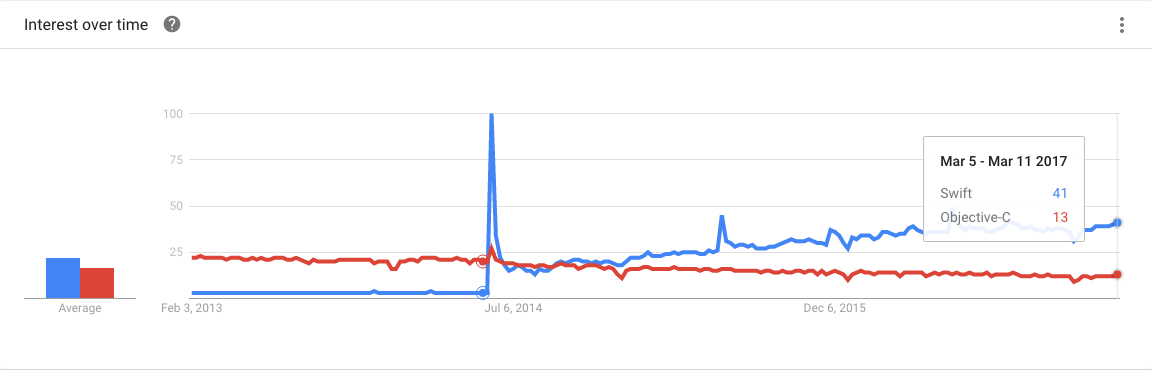
\includegraphics[width=\textwidth]{ObjectiveC-vs-Swift-trend}

\caption{Google trend for searching terms related to Objective C and Swift from Feb 2013 to March 2017}
\label{fig:ObjectiveCVsSwiftTrend}

\end{figure}

The rapid growth of Swift after 2014 can be observed from figure \ref{fig:ObjectiveCVsSwiftTrend}. Its interest index hit the peak on July 2014 when Apple first introduced Swift at \gls{wwdc} and has gradually risen since then. As of the time of writing, Swift possesses an interest rating of 41, three times better than its predecessor. Nevertheless, Swift's powerful and modern set of features is what truly makes it the language choice for this project. Not only Swift eases the developer's life with its interactive environment and errors control system, it also shortens the development span by providing compact syntax and naming convention which leads to better code's readability and reusability.\cite{swift:book} 

Lastly, with the recent addition of Protocol Extension\footnote{Only added since the release of Swift 2.0. Release not is available at: \url{https://developer.apple.com/swift/blog/?id=29}}, Swift officially becomes a \gls{pop} supporting language. Since the main point of this study was to demonstrate the practical use of \gls{pop} and \gls{mvvm} architecture in a real-world project, Swift was an obvious choice over Objective-C.

\section{Presentation Traits - A Better Approach}\label{discussion:betterapproach}
Protocols are blueprints, well-defined contracts and, foremost, abstract instances. They can be easily injected into or ejected from concrete instances. Thus, they should be thought of as pluggable components. In listing \ref{swift:labelTrait}, this characteristic is not demonstrated clearly. Label Trait is a big block and could be still be broken down into several pieces. By further dividing Label Trait into multiple smaller protocols, the code's abstraction level improves greatly. Not only the newly formed protocols can group up to form the original Label Trait, they can also be combined with other protocols to form new Traits if needed. This technique is displayed in listings \ref{css:rootProtocols}, \ref{css:inherit} and \ref{css:result} in appendix \ref{source:code}.

Regarding the code's readability, \gls{pop} is also a great enhancing tool. As mentioned in section \ref{section:pop}, the protocol stands for behaviour. On the other hand, the protocol is verbose, hence its intention is clear and meaningful. By investigating an object and the list of protocols it conforms to, the developer could grab its capability quickly. Perhaps more interestingly, \ref{section:pop} is capable of transforming UI traditional configuration into a \gls{css}-like styling. The source codes listed in appendix \ref{source:code} also demonstrate this progress.

\newpage
\chapter{Conclusion}
Proposals for scalable, maintainable and testable architectures have always sparked broad interest among developers. Concerning this point, \gls{mvp} and \gls{viper} are also interesting topics that have been discussed in a number of articles\footnote{\url{https://medium.com/ios-os-x-development/ios-architecture-patterns-ecba4c38de52}}. From my point of view, a flawless architecture does not exist since they all pose strengths and weaknesses. Additionally, the choice for the architecture should be made unbiased and dependent on specific situations. For instance, although mainstream \gls{mvc} is described as an outdated architecture within the scope of this study, it can still scale up well and be testable if configured correctly\footnote{An example for modern \gls{mvc} base app is available at: \url{https://www.raywenderlich.com/132662/mvc-in-ios-a-modern-approach}}. 

Although the study proposes the practical use of \gls{pop-mvvm}, it does not encourage its readers to hastily apply the model in a real-world project since it is a rather immature and complicated architecture. In my opinion, applying a complex architecture into a real-world project does not necessarily prove one's skill in software development. Rather than that, it is the ability to carry out correct decisions on the use of architecture in different situations. Using a poorly scalable architecture in a large project often results in an unmaintainable code base. Meanwhile, applying a complex model into a simple application is an overkill and not worth the effort spent. All in all, it is not the architecture that prevents its users from testing, scaling or maintaining. The outcomes all lie on the developers' choice. 

On the other hand, this study encourages further reading on the following software principles: \gls{solid} principles and \gls{first} principles. This project could only partly follow the guidelines provided by them, mostly due to my inexperience. However, it proves to be worth the effort since the outcome is a clean, easy to maintain and well documented code base. There are currently a number of articles concerning the practical uses of these principles\footnote{\url{https://github.com/ochococo/OOD-Principles-In-Swift}}$^{,}$\footnote{\url{http://agileinaflash.blogspot.fi/2009/02/first.html}}. 

Last but not least, state of the art is challenging, but not impossible. It cannot be achieved in a day or two, or by a single person. Thus, this study strongly proposes further exploration into the developing and customization of \gls{pop-mvvm}, especially in the Swift language. In the end, it is all up to one's curiosity and creativity that define the characteristics of his/her own architecture.
\chapterprecishere{``True art is characterized by an irresistible urge in the creative artist.``\par\raggedleft--- \textup{Albert Einstein}}

\newpage

%----------------------------------------------------------------------------------------
%   BIBLIOGRAPHY 
%----------------------------------------------------------------------------------------
\IfLanguageName{finnish}{\bibliographystyle{vancouver_fi}}{\bibliographystyle{vancouver}}
%line space
%\singlespacing %removed otherwise the appendix are also single space
\begin{flushleft}
\begin{singlespacing}
\bibliography{biblio}
\end{singlespacing}
\end{flushleft}
%for conting the pages
\label{LastPage}~
\clearpage

\appendix
%\linespread{1.5}
%no page number for appendix in table of content
\addtocontents{toc}{\cftpagenumbersoff{chapter}}
%appendix sections and subsections not in table of content
\settocdepth{chapter}
%add Appendices in the table of content
\addappheadtotoc
%force smaller vertical spacing in table of content
\addtocontents{toc}{\vspace{2pt}}
\pretocmd{\chapter}{\addtocontents{toc}{\protect\vspace{-12pt}}}{}{}
%have Appendix 1 (instead of Appendix A)
\renewcommand{\thechapter}{\arabic{chapter}} 

%special counter for appendix
\setcounter{page}{1}
\newtotcounter{appage1}
%overwrite the header
\makeevenhead{plain}{}{}{Appendix \thechapter \\ \thepage (\stepcounter{appage1}\total{appage1})}
\makeoddhead{plain}{}{}{Appendix \thechapter \\ \thepage (\stepcounter{appage1}\total{appage1})}


\chapter{Using \glspl{trait} to Create \gls{css}-like Styling in Swift} 
This appendix demonstrates the progress of creating the \gls{css}-like styling environment mentioned in section \ref{discussion:betterapproach}. The implementation is copied and modified from Tyler Tillage's article \cite{pop:uikit}.

Firstly, a root protocol is required as seen in listing \ref{css:rootProtocols}. Any class plans to have the \gls{css}-like styling ability must extend this protocol.

\label{source:code}

\begin{listing}[H]
\begin{SwiftCode}
protocol CSSStyling {
    func applyCSSStyling()
}

protocol FontType: CSSStyling {
    var name : String { get }
    var size : CGFloat { get }
    var align : NSTextAlignment { get }
}

protocol Background: CSSStyling {
    var backgroundColor : UIColor { get }
}

protocol Border: CSSStyling {
    var cornerRadius : CGFloat { get }
    var borderWidth : CGFloat { get }
    var borderColor : CGColor { get }
}
\end{SwiftCode}
\caption{Root protocols}
\label{css:rootProtocols}
\end{listing}

As also observed from listing \ref{css:rootProtocols}, a group of styling protocols also inherit from this root. They contain general, abstract attributes and act as the roots of all other specific styling protocols. This inheritance structure is presented in listing \ref{css:inherit}.

\begin{listing}[H]
\begin{SwiftCode}
protocol HeadingFont: FontType{}

extension HeadingFont{
    var name : String {
        return "HelveticaNeue-Bold"
    }
    
    var size : CGFloat {
        return 20.0
    }
    
    var align: NSTextAlignment {
        return NSTextAlignment.center
    }
}

protocol RoundedBorder: Border {}

extension RoundedBorder {
    var cornerRadius: CGFloat {
        return 5.0
    }
    
    var borderWidth: CGFloat {
        return 2.0
    }
    
    var borderColor: CGColor {
        return UIColor.red.cgColor
    }
}

protocol WhiteBackground: Background {}

extension WhiteBackground {
    var backgroundColor: UIColor {
        return UIColor.white
    }
}


\end{SwiftCode}
\caption{Styling protocols}
\label{css:inherit}
\end{listing}

The root styling protocols let their descendants supply their own concrete attributes. As displayed in listing \ref{css:inherit}, the descendant's naming style is similar to \gls{css}'s convention. Furthermore, the attributes are enclosed within the extension scope so as to prevent outer objects from accessing and modifying the original data. These acts provide better readability for new developers as well as withdraws their concerns from the inner implementations. Ultimately, they only need to focus on the actual configuration happens in listing \ref{css:result}.

\begin{listing}[h]
\begin{SwiftCode}
extension UILabel: CSSStyling {
    internal func applyCSSStyling() {
        if let s = self as? FontType {
            self.font = UIFont(name: s.name, size: s.size)
            self.textAlignment = s.align
        }
        
        if let s = self as? RoundedBorder {
            self.layer.borderColor = s.borderColor
            self.layer.borderWidth = s.borderWidth
            self.layer.cornerRadius = s.cornerRadius
        }
        
        if let s = self as? Background {
            self.backgroundColor = s.backgroundColor
        }
    }
}

class HeadingLabel : UILabel, HeadingFont, RoundedBorder, WhiteBackground {
    override init(frame: CGRect) {
        super.init(frame: frame)
        applyCSSStyling()
    }
}

class NormalTextLabel : UILabel, NormalTextFont, RedBackground{}
\end{SwiftCode}
\caption{CSS-like styling for a label}
\label{css:result}
\end{listing}

Detailed implementation for \gls{css} styling is injected into a UILabel's extension, as seen in listing \ref{css:result}. Thus, its subclass only need to conform the preferred attributes. Then, the method for styling (  \mintinline{swift}{applyCSSStyling} in this case) is called within the constructor and the configuration is complete. A \mintinline{swift}{HeadingLabel}'s render is displayed in figure \ref{fig:cssResult_1}. 

\begin{figure}[h]

\centering

\includegraphics[width=0.5\textwidth]{cssResult_1}

\caption{HeadingLabel's render}
\label{fig:cssResult_1}  
\end{figure}

Protocol's verbose power is demonstrated clearly in listing \ref{css:result}. The developer does not waste time looking at the inner codes to predict the appearance of the label. Furthermore, by looking at the \mintinline{swift}{NormalTextFont} declaration in listing \ref{css:result}, the developer expects it to have a red background, no border and a normal font face. The result image is displayed in figure \ref{fig:cssResult_2} to verify these assumptions.

\begin{figure}[h]

\centering
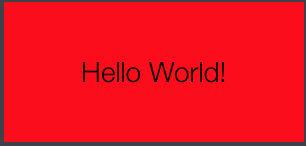
\includegraphics[width=0.5\textwidth]{cssResult_2}

\caption{NormalTextLabel's render}
\label{fig:cssResult_2}  
\end{figure}

Expectations were met and little effort was given. Not only that, this \gls{css}-styling system could be wrapped up into a library and exported for future usage. This system is highly modifiable and requires little documentation or guidance, especially for the case of developers with web development background. 
\end{document}